\documentclass{standalone}
\usepackage[libertine, varg]{newtxmath}
\usepackage[lining]{ebgaramond}
\usepackage{pgfplots}
\begin{document}
	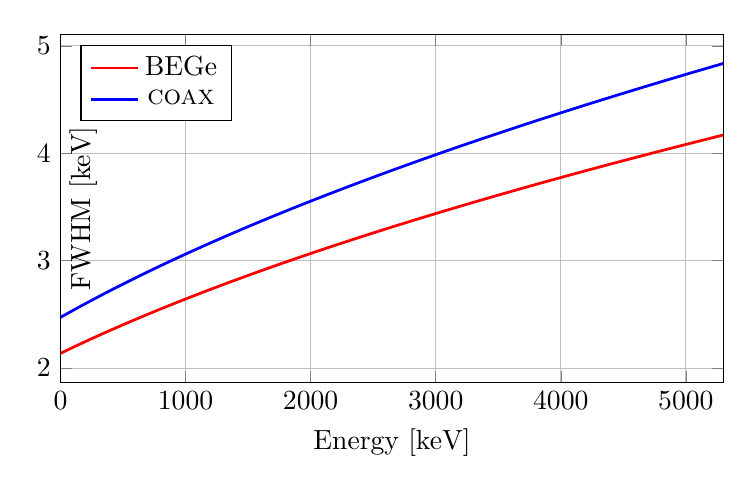
\begin{tikzpicture}
		\begin{axis}[
					%mlineplot,
					width=10cm, height=6cm,
					xmin=0, xmax=5300,
					%ymin=0, ymax=0.6,
					samples=200,
					xlabel=Energy {[}keV{]},
					%yticklabels={,,},
					ylabel=FWHM {[}keV{]},
					grid = major,
					/pgf/number format/1000 sep={},
					ylabel style = {at={(axis description cs:0.07,0.5)}},
					legend entries = {BEGe, \textsc{coax}},
					legend pos = north west,
					]
			\addplot [mark=none, color=red, line width=1pt, domain=0:5300]
			{2.355*sqrt(0.823490+0.000436109*x)};
				%\node at (axis cs:0.3,0.5) {\color{blue}$2\nu\beta\beta$};
			\addplot [mark=none, color=blue, line width=1pt, domain=0:5300]
			{2.355*sqrt(1.10179+x*0.000587762)};
				%\node at (axis cs:1.4,0.35) {\color{red}$2\nu\beta\beta$LV};
		\end{axis}
	\end{tikzpicture}
\end{document}
